\documentclass[10pt,a4paper,arial, spanish]{article}
\usepackage[spanish]{babel}
\usepackage[T1]{fontenc}
\usepackage[utf8]{inputenc}
\usepackage{listingsutf8}
\usepackage{graphicx}
\usepackage{float}
\usepackage{xcolor}
\usepackage[cache=false]{minted}
%\usemintedstyle{borland}
\usepackage[hidelinks, colorlinks=true, linkcolor=blue, urlcolor=blue]{hyperref}

\title{Proyecto Capstone - La Batalla de los Vecindarios (Semana 1)}
\author{R. Salaberry}
%\UseRawInputEncoding
\begin{document}



\maketitle

\begin{abstract}
	Como parte del curso IBM Data Science professional program Capstone Project, trabajaremos con un conjunto de datos reales con el fin de llevar a cabo un proyecto que abarque todas las instancias en las que un científico de datos se encontraría en la vida real al resolver un problema dado.
	
	El principal objetivo de este proyecto es utilizar todas las herramientas vistas en los cursos previos para la resolución de un problema de negocios dado, tal como lo haría en la vida real un científico de datos. 
	
	Se aplicarán los conocimientos adquiridos en la búsqueda de datos, la preparación de los mismos, el análisis y las conclusiones que implican para el caso de negocios planteado.
	El caso de negocio será la apertura de un restaurante de comida sudamericana (cono sur, Argentina, Uruguay, Brasil, Chile y Paraguay) muy populares en la región y que se conocen con el nombre de parrillas o parilladas en la ciudad de Toronto, Canadá. 
	 
	
\end{abstract}


\tableofcontents
\section{Definición del problema}
\subsection{Planteo del problema}
Toronto, una ciudad muy cosmopolita,  es la capital de la provincia de Ontario en Canadá. La ciudad ha albergado tradicionalmente muchas corrientes migratorias que se han establecido con el tiempo en sus barrios, de modo tal que hoy en día existen entre sus barrios, algunos que hacen referencias a la diversidad de culturas de dicha ciudad, como ser Chinatown, Corso Italia, Greektown, Kensington Market, Koreatown, Little India, Little Italy, Little Jamaica y Little Portugal.

% TODO: \usepackage{graphicx} required

\begin{figure}[H]
	\centering
	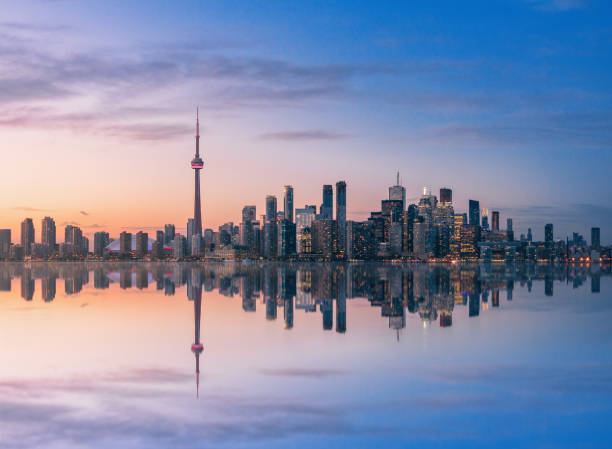
\includegraphics[width=10cm, height=7cm]{Toronto}
	\caption[Ciudad de Toronto]{Ciudad de Toronto, Canadá.}
	\label{fig:toronto}
\end{figure}


En este proyecto, seguiremos paso a paso el proceso para saber si es buena idea la decisión de abrir un restauran de estilo sudamericano en la ciudad de Toronto, cuales son los barrios mas indicados para ello, teniendo en cuenta la migración de origen sudamericano y también los ingresos para cada barrio a fin de  crear para el restauran una clientela con un perfil económico aceptable.

Tomamos como definición de restaurante sudamericano (parrilla o parrillada) aquel en donde se cocina la carne de res a las brasas de la leña en una parilla. La comida típica así definida se denomina asado.

\begin{figure}[h]
	\centering
	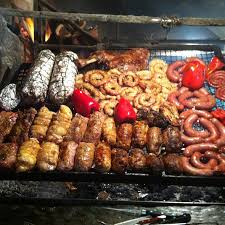
\includegraphics[width=10cm, height=7cm]{parrillada}
	\caption[Parrillada estilo sudamericano]{Parrillada estilo sudamericano}
	\label{fig:parrillada}
\end{figure}

Los países definidos como sudamericanos son los países pertenecientes al denominado cono sur, es decir Argentina, Uruguay, Brasil, Chile y Paraguay. Estos serán la población objetivo  a estudiar y relacionar con los barrios de Toronto.  

Para ello nos planteamos las siguientes preguntas:
\begin{itemize}
	\item  ¿En qué barrios de Toronto vive la comunidad sudamericana del cono sur? 
	\item  ¿Hay restaurantes de estilo sudamericano en Toronto, donde están ubicados? 
	\item  ¿Cómo es la distribución de ingresos de cada barrio de Toronto?
	\item  ¿Cuál es el barrio de Toronto mas apropiado para abrir un restaurante de estilo sudamericano (parrillada) ?  
\end{itemize}
\subsection{Perfil de interesados}
El perfil de personas interesadas en este problema son las personas relacionadas a la comunidad sudamericana de Toronto, y los empresarios sudamericanos que residiendo o no en Toronto deseen invertir en un restaurante típico en la ciudad, así como también cualquier empresario canadiense que quiera invertir en el rubro de gastronomía.

También representa interés a  la comunidad de científicos analistas de datos que deseen analizar los barrios de Toronto para un eventual modelo de negocio del rubro gastronómico.

\section{Fuente de datos. Adquisición y transformación}\label{datos}
Para este planteo vamos a precisar un detalle de los barrios de Toronto, que se puede obtener en Wikipedia desde el siguiente link: {\href{https://en.wikipedia.org/wiki/List_of_postal_codes_of_Canada:_M}{Datos código postal, barrios de Toronto}}. Tambien existe otra pagina con dicha información, es de {\href{https://www.zipcodesonline.com/2020/}{Zipcodesonline}} del año 2020 y tiene los zip codes de muchas ciudades del mundo, entre ellas los de Toronto en este link: {\href{https://www.zipcodesonline.com/2020/06/postal-code-of-toronto-in-2020.html}{Zip code de Toronto}} 

También el siguiente link de {\href{https://cocl.us/Geospatial_data\%E2\%80\%9D}{Coordenadas de códigos postales de Toronto, Canadá}} que proporciona la latitud y longitud de cada uno de los códigos postales que aparecen en la página de wikipedia anterior.

Finalmente vamos a necesitar información demográfica de los barrios de Toronto, esta información la obtenemos del portal de datos de la ciudad de Toronto, {\href{https://open.toronto.ca/dataset/neighbourhood-profiles/}{Datos de perfiles de barrios de Toronto, Canadá}}.

Para obtener la información sobre restaurantes en cada barrio de Toronto, usaremos la API de  {\href{https://developer.foursquare.com/docs}{Foursquare}}. Usando la API obtendremos los nombres, categorías, latitud y longitud de cada restauran existente en cada barrio de Toronto. En esta búsqueda se tratará de ubicar los restaurantes que cumplen con la definición de parrillas o parrilladas de estilo sudamericano.   

\section{Metodología}
Se trabaja con un Notebook Jupyter, realizando el código Python con un kernel Python 3.0.
Los pasos a seguir serán los siguientes:
\begin{itemize}
	\item Pasar a un data frame los datos de los barrios de Toronto de la página de wikipedia.
	\item Relacionar el data frame con las coordenadas latitud y longitud de archivo de coordenadas geográficas trabajado anteriormente.
	\item Obtener la información demográfica relevante de los barrios de Toronto y de la población emigrante de Sudamérica  desde  la base de datos del portal de datos de la ciudad de Toronto.
	\item Combinar los datos demográficos con la base anterior.
	\item Realizar el análisis de los datos para saber donde se ubica la población objetivo.
	\item Obtener datos de restaurantes relacionados (parrilladas) en los barrios de Toronto mediante consultas con la API de Foursquare.
	\item Relacionar la ubicación de dichos restaurantes con la ubicación de la población objetivo.
	\item Analizar los resultados obtenidos y realizar las recomendaciones necesarias.   
\end{itemize}

\section{Desarrollo del trabajo}
De acuerdo al portal de datos de la ciudad de Toronto, existen formalmente en la ciudad 140 barrios,tal como se explica en dicho portal.
Por lo tanto a efectos de este trabajo, tomaremos como base los 140 barrios detallados en el archivo {\href{https://ckan0.cf.opendata.inter.prod-toronto.ca/download_resource/ef0239b1-832b-4d0b-a1f3-4153e53b189e?format=csv}{neighbourhood-profiles-2016-csv}}  que se usa en este trabajo para tomar los datos de migración como se explicó en la sección \ref{datos}.

También en dicho portal se listan los  {\href{https://www.toronto.ca/city-government/data-research-maps/neighbourhoods-communities/neighbourhood-profiles/}{140 barrios reconocidos de Toronto}} que coinciden con los explicados en el párrafo anterior. Por tal motivo, en este trabajo tomamos como barrios de Toronto los 140 que se encuentran en la pagina oficial de datos de Toronto. 

Primero se cargan los paquetes y librerías necesarios.

\begin{minted}[fontsize=\scriptsize,frame=single, breaklines=true, python3=true]{python}
#Importo las librerías paquetes que necesito. Imported the needed library\n",
import re
import numpy as np # librería para manejar datos vectorizados

import pandas as pd # librería para análisis de datos
pd.set_option('display.max_columns', None)
pd.set_option('display.max_rows', None)

import json # librería para manejar archivos JSON 

#!conda install -c conda-forge geopy --yes # retirar el comentario de esta línea si no ha completado el laboratorio de la API de FourSquare 
!pip install geopy
from geopy.geocoders import Nominatim # convertir una dirección en valores de latitud y longitud

import requests # librería para manejar solicitudes
from pandas.io.json import json_normalize # librería para convertir un archivo json en un dataframe pandas

# Matplotlib y módulos asociados para graficar
import matplotlib.cm as cm
import matplotlib.colors as colors

# importar k-means desde la fase de agrupación
from sklearn.cluster import KMeans

#!conda install -c conda-forge folium=0.5.0 --yes # retirar el comentario de esta línea si no ha completado el laboratorio de la API de FourSquare
! pip install folium==0.5.0
import folium # librería para graficar mapas 

# se carga beautiful soup para el trabajo con HTML
! pip install beautifulsoup4
from bs4 import BeautifulSoup

print('Libraries imported.')
\end{minted}
\subsection{Primera parte, los barrios y sus coordenadas}
Luego de cargar las librería a utilizar,  se cargan las tablas en donde esta la información de barrios de Toronto, el postal code y los 140 barrios formales de con el objetivo de obtener un data frame que incluya los 140 barrios con sus respectivas coordenadas de latitud y longitud.

El primer problema surge de ver inconsistencias entre los barrios de la página de wikipedia, los barrios de la página de zipcodesonline y los 140 barrios formales del portal de datos de Toronto, en el cual también se incluye la información demográfica de dichos 140 barrios, por lo tanto, hay que buscar la forma de obtener las coordenadas de los 140 barrios por otro camino.

Se descarta entonces el uso de la información de las paginas de wikipedia y zipcodesonline para buscar las coordenadas a traves del servicio de ``Geolocator'' usado anteriormente para ubicar coordenadas de direcciones.   

Carga de los barrios de la página del portal de datos de la ciudad de Toronto.
\begin{minted}[fontsize=\scriptsize,frame=single, breaklines=true, python3=true]{python}
with open('Neighbourhood Profiles – City of Toronto.html', encoding="utf8") as fp3:
soup = BeautifulSoup(fp3, "html.parser")
table3 = soup.find_all('table')
df3 = pd.read_html(str(table3))[1]
col3 = ['Hood #','Neighborhood']
df3.columns=col3
df3 = df3.reset_index(drop=True)
df3.sort_values(by='Neighborhood')
df3.head()
\end{minted}

Obtenemos el data frame con los 140 barrios. Luego buscamos las coordenadas con el servicio ``Geolocator''.
\begin{minted}[fontsize=\scriptsize,frame=single, breaklines=true, python3=true]{python}
barrio=[]
lat=[]
long=[]
barrio_num=[]
for i in range(len(df3)):
try:
address  = df3.loc[i,'Neighborhood']+','+'Toronto'
geolocator = Nominatim(user_agent="Tor_explorer")
location = geolocator.geocode(address)
latitude = location.latitude
longitude = location.longitude
barrio.append(df3.loc[i,'Neighborhood'])
lat.append(latitude)
long.append(longitude)
barrio_num.append(df3.loc[i,'Hood #'])
except:
barrio_num.append(df3.loc[i,'Hood #'])
barrio.append(df3.loc[i,'Neighborhood'])
lat.append(None)
long.append(None)
col32=['Hood #','Neighborhood', 'Latitude', 'Longitude']
df32=pd.DataFrame(columns=col32)
df32['Hood #']=barrio_num
df32['Neighborhood']=barrio
df32['Latitude']=lat
df32['Longitude']=long
df32.head()\end{minted}
Se recuperan 108 coordenadas de 140 barrios.
\begin{figure}[H]
	\centering
	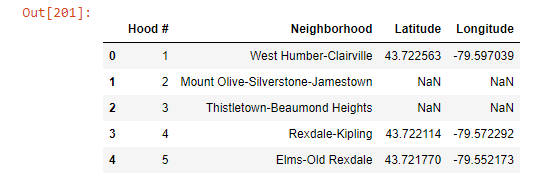
\includegraphics[scale=0.5]{df1}
	\caption[Data frame con coordenadas]{Data frame con coordenadas}
	\label{fig:df1}
\end{figure}

Paso los registros nulos a otro data frame para analizarlos separadamente.
Hay 32 valores Nan correspondientes a barrios de los cuales no se encontraron las coordenadas. Formo otro Data Frame con los barrios que faltan completar y los estudio aparte.

Viendo los vecindarios que quedaron como NaN, la gran mayoría son de dos palabras separadas por ``-''. Luego hay una de una sola palabra (\emph{``Humbermede''} antiguamente \emph{``Emery''}), dos que tienen parentesis (\emph{``Taylor-Massey (formerly Crescent Town)''} y \emph{``Mimico (includes Humber Bay Shores)''} y otros que esta separado por espacios (\emph{``Lambton Baby Point''}, \emph{``Woodbine Corridor''} y \emph{``Parkwoods Donalda''})). Un caso particular es \emph{``Thistletown-Beaumond Heights''}, el cual es mas conocido solo como \emph{``Thistletown''} y por lo tanto se cambia a ese nombre para poder obtener sus coordenadas.

Separo los registros con Nan para estudiarlos separadamente, luego separo los nombres de los barrios para usar su segunda denominación y poder encontrar las coordenadas. También arreglo los casos particulares presentados anteriormente. Luego utilizo de nuevo el servicio ``Geolocator'' para obtener las coordenadas de los restantes barrios. El resultado es un data frame con 32 filas de los barrios que antes eran Nan y ahora tienen su respectivas coordenadas.
\begin{minted}[fontsize=\scriptsize,frame=single, breaklines=true, python3=true]{python}
barrio2=[]
for f in range(len(df32nan)):
n=df32nan.iloc[f,1]
nsplit_aux=re.split('[(]',n)
n2=nsplit_aux[0]
nsplit=re.split('-',n2)
if len(nsplit)>1:
barrio2.append(nsplit[1])
else:
barrio2.append(nsplit[0])
df32nan['Neighborhood2']=barrio2
df32nan
\end{minted}

\begin{minted}[fontsize=\scriptsize,frame=single, breaklines=true, python3=true]{python}
barrio32=[]
lat32=[]
long32=[]
barrio32_num=[]
for i in range(len(df32nan)):
try:
address  = df32nan.loc[i,'Neighborhood2']+','+'Toronto'
geolocator = Nominatim(user_agent="Tor_explorer")
location = geolocator.geocode(address)
latitude = location.latitude
longitude = location.longitude
barrio32_num.append(df32nan.loc[i,'Hood #'])
barrio32.append(df32nan.loc[i,'Neighborhood2'])
lat32.append(latitude)
long32.append(longitude)
except:
barrio32_num.append(df32nan.loc[i,'Hood #'])
barrio32.append(df32nan.loc[i,'Neighborhood2'])
lat32.append(None)
long32.append(None)
df32nan['Hood #']=barrio32_num
df32nan['Neighborhood2']=barrio32
df32nan['Latitude']=lat32
df32nan['Longitude']=long32
df32nan.head()
\end{minted}
Obtengo el data frame con los 32 registros que faltan de los barrios y sus coordenadas. Ahora hay que concatenarlo al otro data frame y obtener así el data frame buscado de los 140 barrios y sus coordenadas.
\begin{figure}[H]
	\centering
	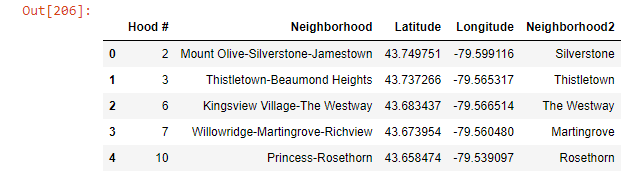
\includegraphics[scale=0.5]{df2}
	\caption[Data frame con coordenadas restante]{Data frame con coordenadas restantes.}
	\label{fig:df2}
\end{figure}

Finalmente elimino la columna de segunda denominación , elimino los Nan del primer data frame y concateno los dos obteniendo el resultado buscado.
\begin{minted}[fontsize=\scriptsize,frame=single, breaklines=true, python3=true]{python}
df32nan=df32nan.drop(['Neighborhood2'], axis=1)
df32=df32.dropna()
df32 = pd.concat([df32, df32nan])
df32 = df32.reset_index(drop=True)
print(df32.shape)
df32.head()
\end{minted}

Obtengo el siguiente data frame:
\begin{figure}[h]
	\centering
	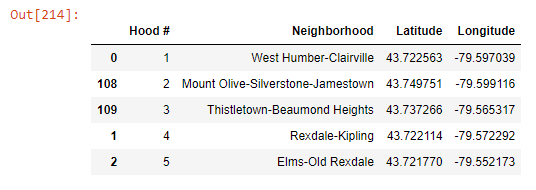
\includegraphics[scale=0.5]{df3}
	\caption[Data frame final.]{Data frame final con los 140 barrios y sus coordenadas.}
	\label{fig:df3}
\end{figure}

Finalmente creamos un mapa para ver los resultados de los 140 barrios de Toronto.
\begin{minted}[fontsize=\scriptsize,frame=single, breaklines=true, python3=true]{python}
# crear un mapa de Toronto utilizando los valores de latitud y longitud
map_toronto = folium.Map(location=[latitude, longitude], zoom_start=10)
# añadir marcadores al mapa
for lat, lng, neighborhood, hood in zip(df32['Latitude'], df32['Longitude'], df32['Neighborhood'],df32['Hood #'] ):
label = '{}, hood n° {}'.format(neighborhood, hood)
label = folium.Popup(label, parse_html=True)
folium.CircleMarker(
[lat, lng],
radius=5,
popup=label,
color='blue',
fill=True,
fill_color='#3186cc',
fill_opacity=0.7,
parse_html=False).add_to(map_toronto)  

map_toronto
\end{minted}
\begin{figure}[h]
	\centering
	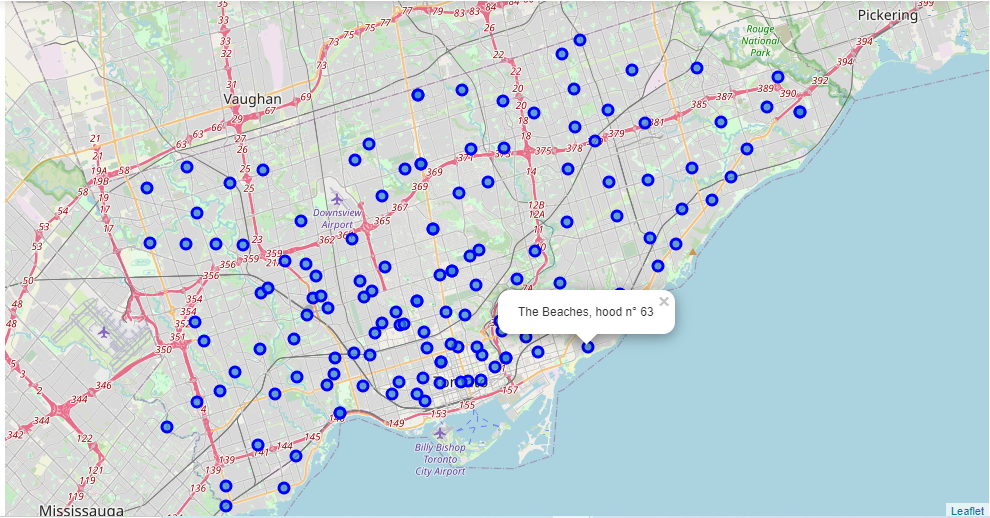
\includegraphics[scale=0.45]{map1}
	\caption[Barrios de Toronto.]{Barrios de Toronto.}
	\label{fig:map1}
\end{figure}

\subsection{Segunda parte, datos demográficos de residentes sudamericanos}
Comenzamos cargando el archivo csv bajado del portal de datos de la ciudad de Toronto. Despues de un estudio de sus características, buscamos con las palabras claves \emph{Neighbourhood Number , Total income: Average amount (\$), Brazil, Brazilian, Argentinian, Chilean, Paraguayan, y Uruguayan} para filtrar los valores que nos interesan.
\begin{minted}[fontsize=\scriptsize,frame=single, breaklines=true, python3=true]{python}
df_demo=pd.read_csv('neighbourhood-profiles-2016-csv.csv',decimal=",") 
valores_a_buscar=['Neighbourhood Number',
'Total income: Average amount ($)',
'Brazil', 
'Brazilian', 
'Argentinian',
'Chilean',
'Paraguayan',
'Uruguayan']
[True if item in df_demo.values else False for item in valores_a_buscar] 
\end{minted}
Como los datos son todos interpretados como strings y ademas los numeros tiene comas, limpiamos la base para poder analizarla

\begin{minted}[fontsize=\scriptsize,frame=single, breaklines=true, python3=true]{python}
demo2 = df_demo2.reset_index(drop=True)
columns=df_demo2.columns
for i in range(1,len(columns),1):
df_demo2.iloc[8,i] = df_demo2.iloc[8,i].replace(",", "")
val=df_demo2.iloc[8,i]
df_demo2.iloc[8,i] = pd.to_numeric(val, errors='coerce')
df_demo2.iloc[1,i] = pd.to_numeric(df_demo2.iloc[1,i], errors='coerce')
df_demo2.iloc[2,i] = pd.to_numeric(df_demo2.iloc[2,i], errors='coerce')
df_demo2.iloc[1,:]=df_demo2.iloc[1,:]+df_demo2.iloc[2,:]
df_demo2=df_demo2.drop(2, axis=0)
df_demo2 = df_demo2.reset_index(drop=True)
for f in range(len(df_demo2.index)):
for c in range(1,len(columns),1):
df_demo.iloc[f,c]=pd.to_numeric(df_demo.iloc[f,c], downcast='integer',errors='coerce')
df_demo2  
\end{minted}
Luego trasponemos el data frame y hacemos lo necesario para calcular la suma de sudamericanos por barrio y poder trabajarlos como un todo.
\begin{minted}[fontsize=\scriptsize,frame=single, breaklines=true, python3=true]{python}
df_demo22=df_demo2.transpose()
df_demo22 = df_demo22.rename_axis('index').reset_index()
fila0=df_demo22.loc[0,:]
df_demo22.columns=fila0
df_demo22=df_demo22.drop(0,axis=0)
df_demo22 = df_demo22.reset_index(drop=True)
df_demo22 = df_demo22.rename(columns={'Characteristic':'Neighborhood',
'Neighbourhood Number':'Hood #',
'BrazilBrazil':'Brazil'})
df_demo22.head()
\end{minted}
\begin{minted}[fontsize=\scriptsize,frame=single, breaklines=true, python3=true]{python}
filas=df_demo22.index
colu=df_demo22.columns
len(filas), len(colu)
for f in range(len(filas)):
for c in range(1, len(colu)-2,1):
df_demo22.iloc[f,c]=pd.to_numeric(df_demo22.iloc[f,c], downcast='integer',errors='coerce')
df_demo22['Total migrantes sudamericanos']=df_demo22.iloc[:,-7:-2].sum(axis=1)
df_demo22 = df_demo22.reset_index(drop=True)
\end{minted}
Obtenemos el siguiente data frame:
\begin{figure}[h]
	\centering
	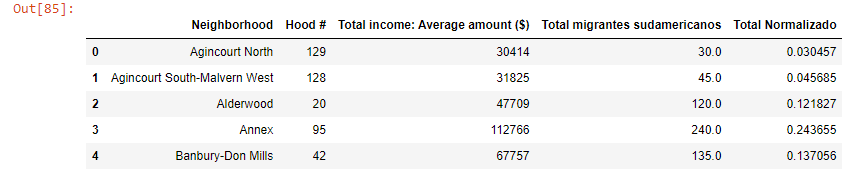
\includegraphics[scale=0.5]{df4}
	\caption[Data frame final de datos demográficos.]{Data frame final de datos demográficos.}
	\label{fig:df4}
\end{figure}
Finalmente hacemos un merge de ambos data frames y tenemos la información necesaria con la ubicación geográfica para cada barrio. En total quedaron 140 barrios.
\begin{minted}[fontsize=\scriptsize,frame=single, breaklines=true, python3=true]{python}
df_demo=df_demo.merge(df_coor,how='inner',on=['Hood #'])
df_demo.head()
\end{minted}
\begin{figure}[h]
	\centering
	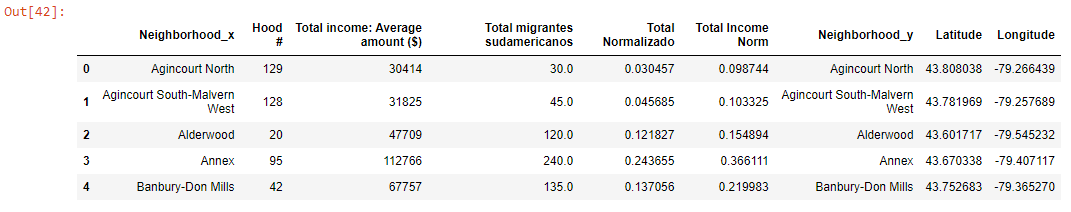
\includegraphics[scale=0.4]{df5}
	\caption[Data frame final de datos demográficos y coordenadas.]{Data frame final de datos demográficos y coordenadas.}
	\label{fig:df5}
\end{figure}

\subsection{Tercera parte. Análisis primario de los datos demográficos }
Para visualizar los datos hacemos un mapa que sea proporcional a la cantidad de migrantes sudamericanos en color rojo, ajustando el radio para tal motivo, y en azul proporcional a los ingresos de cada barrio.
\begin{minted}[fontsize=\scriptsize,frame=single, breaklines=true, python3=true]{python}
# crear un mapa de Toronto utilizando los valores de latitud y longitud
map_toronto2 = folium.Map(location=[latitude, longitude], zoom_start=10)
# añadir marcadores al mapa
for lat, lng, neighborhood, hood, radio, pop, radioincome, income in zip(df_demo['Latitude'], df_demo['Longitude'], 
df_demo['Neighborhood_x'],df_demo['Hood #'],
df_demo['Total Normalizado'],df_demo['Total migrantes sudamericanos'],
df_demo['Total Income Norm'],df_demo['Total income: Average amount ($)']):
label1 = '{}, hood n° {}, pop. {} '.format(neighborhood, hood, pop)
label1 = folium.Popup(label1, parse_html=True)
label2 = '{}, hood n° {}, Income. {} '.format(neighborhood, hood, income)
label2 = folium.Popup(label2, parse_html=True)

folium.CircleMarker(
[lat, lng],
radius=1,
#popup=label,
color='red',
fill=True,
fill_color='#3186cc',
fill_opacity=0.7,
parse_html=False).add_to(map_toronto2)
folium.Circle(
radius=radio*500,
popup=label1,
location=[lat,lng],
color='red',
fill=True,
fill_color='red'
).add_to(map_toronto2) 
folium.CircleMarker(
[lat, lng],
radius=1,
#popup=label,
color='blue',
fill=True,
fill_color='#3186cc',
fill_opacity=0.7,
parse_html=False).add_to(map_toronto2)
folium.Circle(
radius=radioincome*500,
popup=label2,
location=[lat,lng],
color='blue',
fill=True,
fill_color='blue'
).add_to(map_toronto2)     
\end{minted}
\begin{figure}[h]
	\centering
	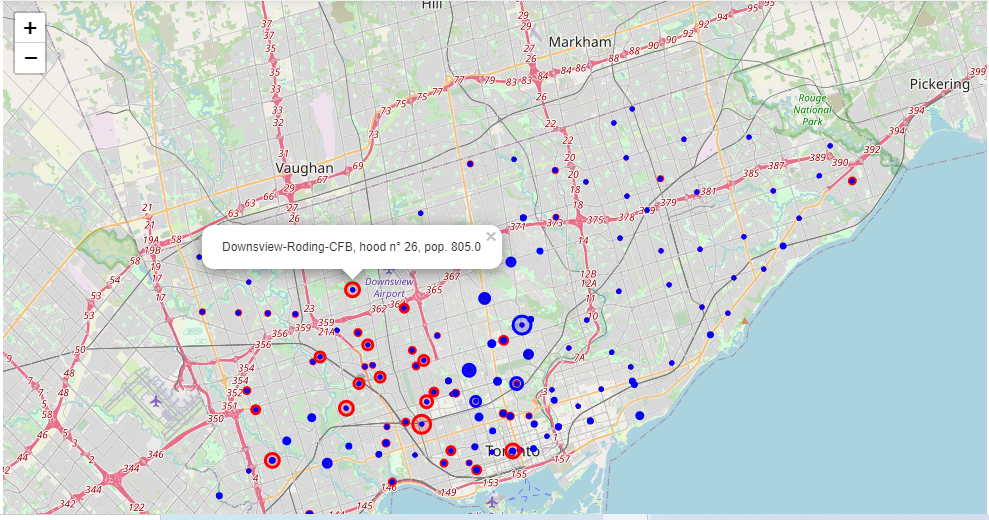
\includegraphics[scale=0.45]{map2}
	\caption[Barrios de Toronto y población sudamericana.]{Barrios de Toronto y población sudamericana.}
	\label{fig:map2}
\end{figure}

Los círculos rojos mas grandes muestra la mayor concentración de migrantes sudamericanos, y los círculos azules mas grandes la mayor concentración de ingresos.

Para poder hacer una agrupación adecuada, es preciso estudiar cual será el número de klusters ideal, hacemos este estudio usando el método Elbow.
\begin{minted}[fontsize=\scriptsize,frame=single, breaklines=true, python3=true]{python}
df_demo2=df_demo
toronto_grouped_clustering = df_demo2.drop(['Neighborhood_x','Neighborhood_y', 'Hood #', 
'Total Normalizado','Total Income Norm'], 1)
from sklearn import metrics
from scipy.spatial.distance import cdist

kmeans_kwargs = {"init": "k-means++","n_init": 10,"max_iter": 300,"random_state": 0,}
# A list holds the SSE values for each k
sse = []
for k in range(1, 11):
kmeans = KMeans(n_clusters=k, **kmeans_kwargs)
kmeans.fit(toronto_grouped_clustering)
sse.append(kmeans.inertia_)
plt.style.use("fivethirtyeight")
plt.plot(range(1, 11), sse)
plt.xticks(range(1, 11))
plt.xlabel("Number of Clusters")
plt.ylabel("SSE")
plt.show()
\end{minted}
La gráfica obtenida muestra que el número ideal de kluster es 3.
\begin{figure}[H]
	\centering
	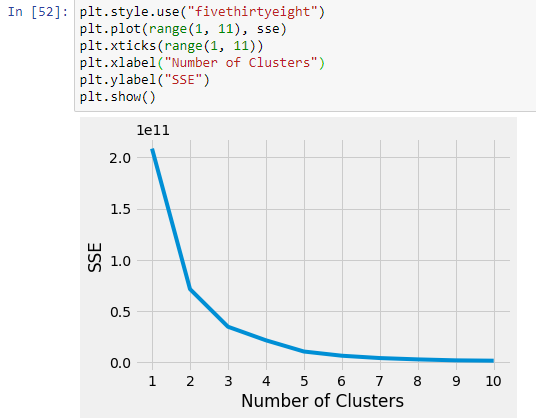
\includegraphics[scale=0.45]{graf1}
	\caption[Número ideal de Klusters.]{Número ideal de Klusters.}
	\label{fig:graf1}
\end{figure}



%---------------
Vamos a probar con 3 klusters para visualizar distinto, incluyendo el ingreso medio por barrio.
\begin{minted}[fontsize=\scriptsize,frame=single, breaklines=true, python3=true]{python}
# establecer el número de agrupaciones
df_demo2=df_demo
kclusters = 3

toronto_grouped_clustering = df_demo2.drop(['Neighborhood_x','Neighborhood_y', 'Hood #', 
'Total Normalizado','Total Income Norm'], 1)

# ejecutar k-means
kmeans = KMeans(n_clusters=kclusters, random_state=0).fit(toronto_grouped_clustering)

# revisar las etiquetas de las agrupaciones generadas para cada fila del dataframe
kmeans.labels_[0:10] 
\end{minted}

Luego llevamos los klusters al mapa.
\begin{minted}[fontsize=\scriptsize,frame=single, breaklines=true, python3=true]{python}
# crear mapa
map_clusters = folium.Map(location=[latitude, longitude], zoom_start=11)

# establecer el esquema de color para las agrupaciones
x = np.arange(kclusters)
ys = [i + x + (i*x)**2 for i in range(kclusters)]
colors_array = cm.rainbow(np.linspace(0, 1, len(ys)))
rainbow = [colors.rgb2hex(i) for i in colors_array]

# añadir marcadores al mapa
markers_colors = []
for lat, lon, poi, cluster, radio in zip(df_demo2['Latitude'], df_demo2['Longitude'],
df_demo2['Neighborhood_x'], df_demo2['Cluster Labels'], df_demo2['Total Normalizado']):
label = folium.Popup(str(poi) + ' Cluster ' + str(cluster), parse_html=True)
folium.CircleMarker(
[lat, lon],
radius=10*radio,
popup=label,
color=rainbow[cluster-1],
fill=True,
fill_color=rainbow[cluster-1],
fill_opacity=0.7).add_to(map_clusters)
\end{minted}

Obtenemos el siguiente mapa:
\begin{figure}[H]
	\centering
	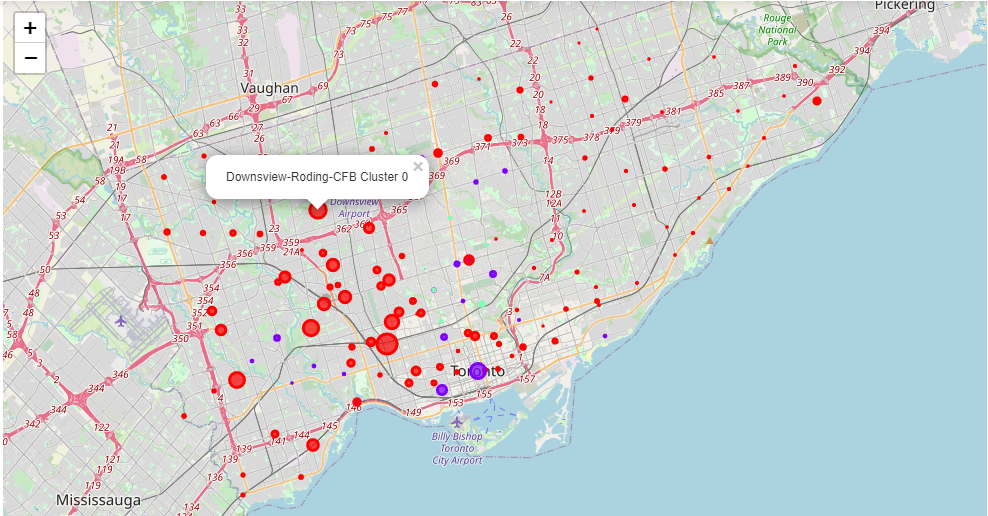
\includegraphics[scale=0.45]{map3}
	\caption[Klusters de barrios por densidad de migrantes sudamericanos.]{Klusters de barrios por densidad de migrantes sudamericanos.}
	\label{fig:map3}
\end{figure}

Miramos la información obtenida en forma de tabla.

\begin{minted}[fontsize=\scriptsize,frame=single, breaklines=true, python3=true]{python}
for i in range(0,3,1):
print('Cluster {}, ingreso medio {}, población sudamericana media {}, cantidad barrios {} '.format(
df_demo2.loc[df_demo2['Cluster Labels'] == i].mean()[0], df_demo2.loc[df_demo2['Cluster Labels'] == i].mean()[2],
df_demo2.loc[df_demo2['Cluster Labels'] == i].mean()[3], df_demo2.loc[df_demo2['Cluster Labels'] == i].count()[1]))
\end{minted}
\begin{tabular}{|c|c|c|c|}
	\hline
	Cluster & Ingreso medio & Población sudamericana media  & cantidad barrios  \\
	\hline    
	0.0 & 41146.23 & 206.32   & 113  \\
	\hline
	1.0 & 92299.09 & 165.22   & 22  \\
	\hline
	2.0 & 210936.8 & 113.0 & 5   \\
	\hline

\end{tabular}

Una primera conclusión es que en el kluster donde mayor es el ingreso promedio, es menor la concentración de sudamericano, y donde la concentración es mayor, el ingreso promedio es el mínimo.

\subsection{Cuarta parte. Obtención de datos de restaurantes sudamericanos }
En esta parte trabajamos con la API de Foursquare para obtener datos sobre negocios de Toronto, pero particularmente de restaurantes de comida típica sudamericana.

Primero fijamos los datos para la API. 

\begin{minted}[fontsize=\scriptsize,frame=single, breaklines=true, python3=true]{python}
CLIENT_ID = 'TKDEL1UDPMTSHP2J0DTMAMEJAXWSZOT1EHMVGYQHE5Z1XYXG' # su ID de Foursquare
CLIENT_SECRET = 'BZSEZJINU52JACXRQMH5A0PZBZMMV2HFF4XP1F2G0TKOJ32M' # Secreto de Foursquare
VERSION = '20210709' # versión de la API de Foursquare
LIMIT = 100 # Un valor límite para la API de Foursquare

print('Your credentails:')
print('CLIENT_ID: ' + CLIENT_ID)
print('CLIENT_SECRET:' + CLIENT_SECRET)
\end{minted}
Con la función \emph{getNearbyVenues} obtenemos todos los datos de negocios de cada barrio.
\begin{minted}[fontsize=\scriptsize,frame=single, breaklines=true, python3=true]{python}
def getNearbyVenues(names, latitudes, longitudes, radius=500):

venues_list=[]
for name, lat, lng in zip(names, latitudes, longitudes):
print(name)

# crear la URL de solicitud de API
url = 'https://api.foursquare.com/v2/venues/explore?&client_id={}&client_secret={}&
v={}&ll={},{}&radius={}&limit={}'.format(
CLIENT_ID, 
CLIENT_SECRET, 
VERSION, 
lat, 
lng, 
radius, 
LIMIT)

# solicitud GET
results = requests.get(url).json()["response"]['groups'][0]['items']

# regresa solo información relevante de cada sitio cercano
venues_list.append([(
name, 
lat, 
lng, 
v['venue']['name'], 
v['venue']['location']['lat'], 
v['venue']['location']['lng'],  
v['venue']['categories'][0]['name']) for v in results])

nearby_venues = pd.DataFrame([item for venue_list in venues_list for item in venue_list])
nearby_venues.columns = ['Neighborhood', 
'Neighborhood Latitude', 
'Neighborhood Longitude', 
'Venue', 
'Venue Latitude', 
'Venue Longitude', 
'Venue Category']

return(nearby_venues)
\end{minted}

\begin{figure}[h]
	\centering
	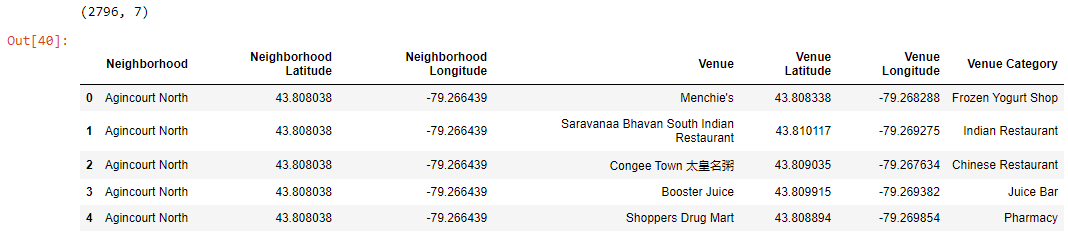
\includegraphics[scale=0.4]{df6}
	\caption[Datos de API de Foursquare.]{Datos de API de Foursquare.}
	\label{fig:df6}
\end{figure}
Hago una lista con las categorías de negocios encontradas y busco con el criterio de denominación sudamericana para un restaurante.


\begin{minted}[fontsize=\scriptsize,frame=single, breaklines=true, python3=true]{python}
venues_cat=toronto_venues['Venue Category'].tolist()
search_list = [ 'Argentinian', 'Brazilian', 'Uruguayan', 'Chilean', 'Paraguayan', 
'Parrilla', 'Parrillada', 'Asado', 'Asador']
len(search_list), type(search_list)
for i in range(len(venues_cat)):
for j in range(len(search_list)):
if search_list[j] in venues_cat[i]:
print(search_list[j], search_list.index(search_list[j]), venues_cat[i], venues_cat.index(venues_cat[i]) )
else:
pass
toronto_venues2=toronto_venues[(toronto_venues['Venue Category'] =='Argentinian Restaurant')
| (toronto_venues['Venue Category'] =='Brazilian Restaurant')]
toronto_venues2
\end{minted}
Se encuentra solo dos restaurantes de estilo sudamericano.
\begin{figure}[h]
	\centering
	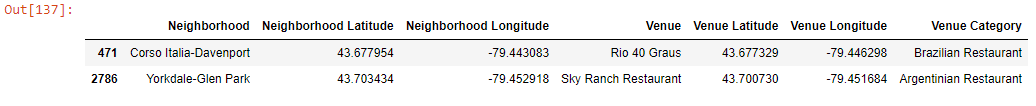
\includegraphics[scale=0.4]{df7}
	\caption[Restaurantes de estilo sudamericano.]{Restaurantes de estilo sudamericano.}
	\label{fig:df7}
\end{figure}
Finalmente grafico sobre el mapa de klusters para ver la ubicación de los restaurantes.


\begin{minted}[fontsize=\scriptsize,frame=single, breaklines=true, python3=true]{python}
# crear mapa
map_clusters2 = folium.Map(location=[latitude, longitude], zoom_start=11)

# establecer el esquema de color para las agrupaciones
x = np.arange(kclusters)
ys = [i + x + (i*x)**2 for i in range(kclusters)]
colors_array = cm.rainbow(np.linspace(0, 1, len(ys)))
rainbow = [colors.rgb2hex(i) for i in colors_array]

# añadir marcadores al mapa
markers_colors = []
for lat, lon, poi, cluster, radio in zip(df_demo2['Latitude'], df_demo2['Longitude'],
df_demo2['Neighborhood_x'], df_demo2['Cluster Labels'], df_demo2['Total Normalizado']):
label = folium.Popup(str(poi) + ' Cluster ' + str(cluster), parse_html=True)
folium.CircleMarker(
[lat, lon],
radius=10*radio,
popup=label,
color=rainbow[cluster-1],
fill=True,
fill_color=rainbow[cluster-1],
fill_opacity=0.7).add_to(map_clusters2)

for venlat, venlon, vencat, venue, nei in zip(toronto_venues2['Venue Latitude'], toronto_venues2['Venue Longitude'],
toronto_venues2['Venue Category'], toronto_venues2['Venue'], 
toronto_venues2['Neighborhood']):
label = folium.Popup(venue + ' ' + vencat , parse_html=True)
folium.Marker([venlat, venlon],popup=label).add_to(map_clusters2) 
\end{minted}
\begin{figure}[H]
	\centering
	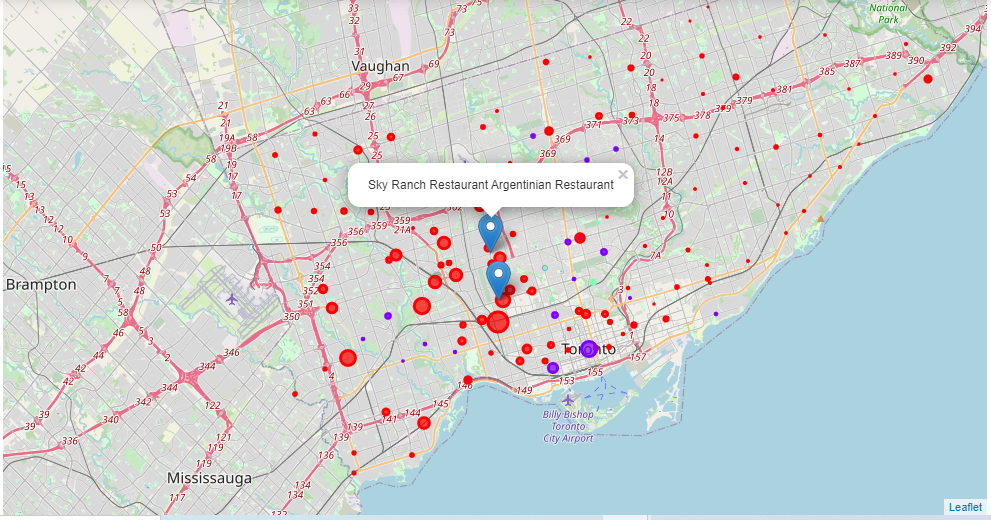
\includegraphics[scale=0.45]{map4}
	\caption[Klusters de barrios por densidad de migrantes sudamericanos y restaurantes de estilo.]{Klusters de barrios por densidad de migrantes sudamericanos y restaurantes de estilo.}
	\label{fig:map4}
\end{figure}
Finalmente analizamos cada kluster para ver la información de población sudamericana e ingresos junto al mapa que tiene la ubicación de los restaurantes.

\begin{figure}[H]
	\centering
	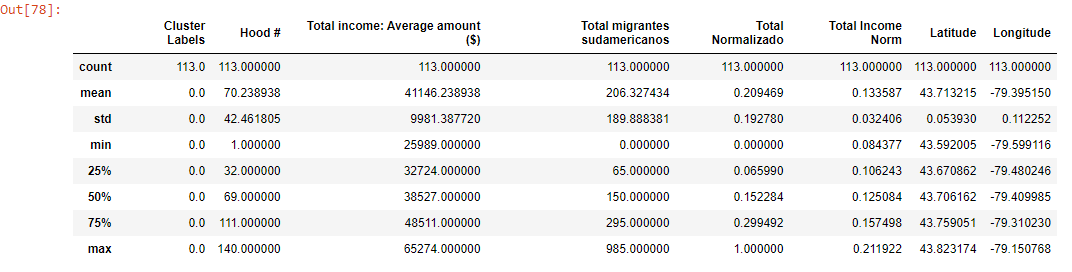
\includegraphics[scale=0.45]{df8}
	\caption[Características del Klusters 0.]{Características del Klusters 0.}
	\label{fig:df8}
\end{figure}
\begin{figure}[H]
	\centering
	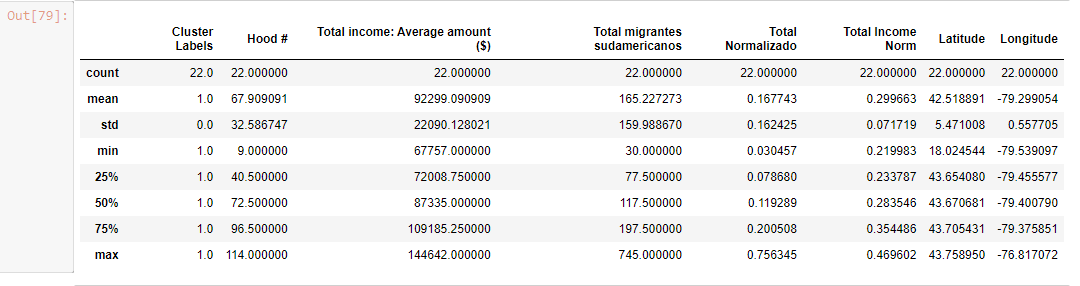
\includegraphics[scale=0.45]{df9}
	\caption[Características del Klusters 1.]{Características del Klusters 1.}
	\label{fig:df9}
\end{figure}
\begin{figure}[H]
	\centering
	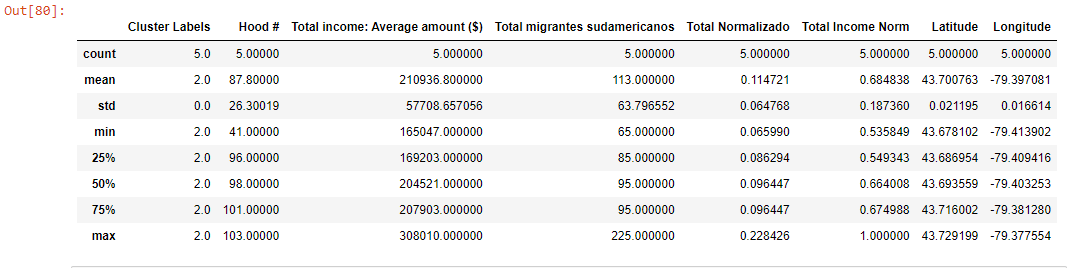
\includegraphics[scale=0.45]{df10}
	\caption[Características del Klusters 2.]{Características del Klusters 2.}
	\label{fig:df10}
\end{figure}

\section{Resultados}
Luego del detallado análisis hecho sobre la comunidad migrante sudamericana de Toronto y los restaurantes de comida típica de dicha comunidad, podemos deducir lo siguiente:
\begin{itemize}
	\item La población migrante sudamericada está distribuida mayoritariamente dentro del kluster 0 de 113 barrios de Toronto.
	\item Existen solo dos restaurantes típicos sudamericanos en el área de Toronto, los mismos están ubicados en una área de mayor concentración de migrantes.Es el área de kluster 0 e incluye 113 barrios.
	\item Dicha área es la de menor ingreso promedio (\$41146.23) de todas las agrupaciones obtenidas en el estudio.
	\item Las área de mayor ingreso son las de menor migración sudamericana promedio y las de mayor concentración son las de menores ingresos.
\end{itemize} 

\section{Conclusiones}
Podemos concluir del análisis realizado lo siguiente:
\begin{itemize}
	\item Dado la escasa cantidad de restaurantes de comida típica sudamericana, recomendamos la ubicación de dicho tipo de restaurantes en las áreas del kluster 2, que se encuentra contigua a la del kluster 0 (con mayor proporción de migrantes sudamericanos) pero con un ingreso medio bastante mayor.
	\item De todos modos, dada que solo existen dos restaurantes de este tipo, la ventana de oportunidad para la apertura de dicho tipo de restaurantes es bastante grande, con posibilidades de éxito mayor si se ubica en la zona recomendada en el punto anterior.
	\item Este análisis presenta algunos punto débiles que son:
	\subitem Los kluster se basan en la información del censo 2016, y por lo tanto hay una brecha de actualización de información de 5 años.
	\subitem Los datos de restaurantes típicos sudamericanos se basan unicamente en los datos de obtenidos de Foursquare API, lo cual podrían no ser ni actualizados ni completos.
	\item A pesar de que se pueden mejorar en los aspectos anteriores, este análisis ciertamente nos ha brindado una primera imagen del problema planteado, pudiendo contestar las preguntas planteadas inicialmente, aunque puede mejorarse el mismo con mayor y mejor información.
	\item En este proyecto tuvimos la oportunidad de abordar un problema empresarial como lo haría un científico de datos real. Usamos muchas bibliotecas de Python para obtener los datos, manipular los contenidos y analizar y visualizar esos conjuntos de datos. Usamos la API de Foursquare para explorar los negocios en los vecindarios de Toronto y buscar aquellos que nos interesaban. Usamos también datos del portal de datos de la Ciudad de Toronto, usamos las librerías seaborn, matplotlib y Folium para visualizar los datos en un mapa. También pudimos usar algoritmos de clasificación como K-means para agrupar los barrios con criterios apropiados.
	\item Hemos hecho uso de todas las herramientas aprendidas para resolver un problema de ciencia de datos real, el mismo puede extenderse a otros problemas similares como abrir gimnasios, tiendas de artesanías, copra de inmuebles, etc. Este proyecto constituye así una guía inicial para abordar mayores desafíos de ciencia de datos en la vida real.
\end{itemize} 


\end{document}
